\section{Systemkontext}
\label{sec:system_context}
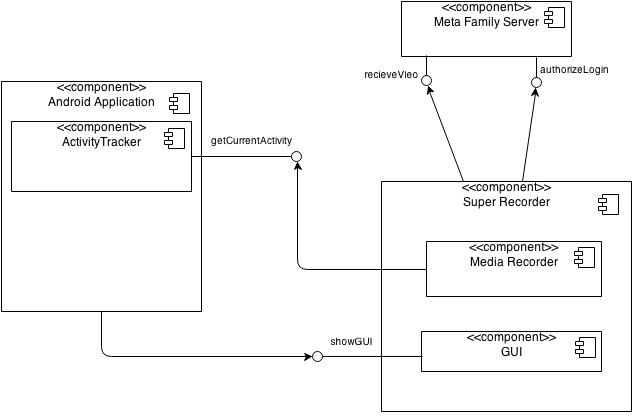
\includegraphics[width=\linewidth]{UML3.jpg}
Super Recorder är del av två externa system; Beta Familys serversida samt de applikationer som implementerar SDK:t. De applikationer som implementerar SDK:t anropar endast metoder för att ta fram och visa GUI:t emedan SDK:t endast anropar applikationerna för att hämta den nuvarande Activityn (vilket är ett centralt objekt för att kunna spela in applikationen). Då detta är den enda kontakten mellan dessa två system är denna relation väldigt loose couplad. 
Gentemot Beta Familys server är det även där en mycket begränsad mängd kommunikation. Super Recorder skickar videoinformation i kombination med att användaren laddar upp en testsession samt verifierar inloggning när en användare vill logga in. 

\subsection{Applikationer}
Den SDK som projektgruppen utvecklar kommer att ha en tät integration med applikationen den används i. Det är fortfarande inte klart huruvida utvecklaren själv behöver ändra sin källkod för att implementera denna ScreenRecorder eller om ett skript kommer köras som automatiskt placerar kodstycken på rätt plats. Detta gör det svårt att förutse vilket gränssnitt som kommer erbjudas utvecklarna. Förhoppningen är att detta gränssnitt ska vara så simpelt som möjligt.

\subsection{Server}
När ett test genomförts kommer en mängd filer ha genererats. Detta är informationen om testet som kommer att användas för att rendera en testningsvideo. SDK:t kommer alltså innehålla ett gränssnitt gentemot servern för överföring av dessa filer. 